
\documentclass[svgnames, 11pt]{report}
 
\usepackage[left=2.5cm, right=2.5cm]{geometry}   % set margins
\usepackage[utf8]{inputenc}                      % set input encoding to utf8
\usepackage{tikz}                                % tikz drawing library
\usepackage{kpfonts}                             % kpfonts
\usepackage[explicit]{titlesec}                  % titlesec
\usepackage{hyperref}                            % use \url
\usepackage{ifthen}                              % \ifthenelse{condition}{if valid}{if not valid}
\usepackage{float}                               % avoid tables/figures to "float away" with [H]
\usepackage{titling}                             % use \thetitle, \thedate, osv
\usepackage{graphicx}                            % used to include graphics

% Use tikx libraries
\usetikzlibrary{shadows.blur}
\usetikzlibrary{shapes.symbols}

% Define space between sections
\newcommand{\secspace}{0.5cm}

% Define chapter style
\newcommand*\chapterlabel{}
\titleformat{\chapter}
  {\gdef\chapterlabel{}
   \normalfont\sffamily\Huge\bfseries\scshape}
  {\gdef\chapterlabel{}}{0pt}               % change to \chapterlabel{\thechapter\ } to display numbering in title
  {\begin{tikzpicture}[remember picture,overlay]
    \node[yshift=-3.0cm, xshift=1.1cm] at (current page.north west)
      {\begin{tikzpicture}[remember picture, overlay]
        \draw[top color=red, bottom color=DarkRed, blur shadow] (0,0) rectangle
              (2cm,3cm);
        \node[yshift=0.7cm, xshift=1cm, scale=2]
              {\color{white}
                \ifthenelse{\thechapter < 1} % if \thechapter < 1, display nothing
                {}
                {\thechapter}};
        \node[anchor=west, yshift=0.35cm, xshift=2cm]
              {\color{black}\chapterlabel#1};
       \end{tikzpicture}
      };
   \end{tikzpicture}
  }
\titlespacing*{\chapter}{0pt}{50pt}{-60pt}

% Define section style
\titleformat{\section}[block]
  {\huge\bfseries
    \tikz[overlay] \shade[left color=DarkRed,right color=red, blur shadow] (0,-1ex) rectangle (\textwidth,1em);}%    
  {\color{white}\ \thesection}
  {1em}
  {\color{white}#1}

% Define subsection style
\titleformat{\subsection}[block]%
  {\LARGE\bfseries
    \tikz[overlay] \shade[left color=DarkRed,right color=red, blur shadow] (0,-1ex) rectangle (\textwidth,1em);}%    
  {\color{white}\ \thesubsection}
  {1em}
  {\color{white} #1}

% Define title, author and date
\title{Technical Report}
\author{\Large Anders \textsc{Strand} \\
        \Large Emil Taylor \textsc{Bye} \\
        \Large Petter S. \textsc{Storvik} \\
        \Large Odd M. \textsc{Trondrud} \\
        \Large Ole \textsc{Bauck}}
\date{\today}

% Document
\begin{document}

% Titlepage
% Titlepage
\begin{titlepage}
\begin{tikzpicture}[remember picture,overlay]
    \node[yshift=-10cm, xshift=0.01cm] at (current page.north west)
      {\begin{tikzpicture}[remember picture, overlay]
           \draw[top color=Blue, bottom color=DarkBlue] (0,0) rectangle
                (\paperwidth-0.02cm,10cm);
           \node[anchor=west, yshift=3cm, xshift=2cm, scale=0.2cm]
                {\color{white} \thetitle};
           \node[anchor=west, yshift=0.5cm, xshift=17cm, scale=1.5]
                {\color{white} \thedate};
           \node[anchor=west, yshift=-5cm, xshift=2.7cm, align=left]
                {\color{black} \theauthor};
           \node[yshift=-14.5cm, xshift=11cm, align=center]
                {\color{black}\large Eksperter i Team};
           \node[yshift=-15cm, xshift=11cm, align=center]
                {\color{black}\large TMM4850 - Instrumentering og styring over internett};
           \node[yshift=-15.5cm, xshift=11cm, align=center]
                {\color{black}\large Norges Teknisk-Naturvitenskapelige Universitet};
       \end{tikzpicture}
      };
   \end{tikzpicture}
\end{titlepage}


% Abstract
\chapter{Abstract}
Abstract analysis goes here

% ToC
\tableofcontents

% Introduction
\chapter{Introduction}
%TODO: Noen andre enn Odd må gå gjennom dette.
Our group was assigned to the ``Instrumentering og Styring over nett'' village, which has a focus on remote control over the internet.
The tackled problem can be summarized as follows:
\begin{quote}
Construct a platform that facilitates instrumentation and remote control over the internet.
Demonstrate its feasibility by remote controlling a car-like robot with sensors, a camera and actuators.
The platform should be modular and security should be focused on during the development process.
\end{quote}

We decided to build a platform to facilitate the communication between operators and the devices they wish to remote control over the internet.
Devices connected to the platform should have their functionality, available commands and sensory readings made available to authorized users through the platform.
The platform should be modular in order to more easily allow the adding of functionality to meet domain specific requirements.
It should also meet typical security requirements: Eavesdropping on the communication should not be possible and some secure authorization scheme should be supported in order to restrict access to devices connected to the platform.

Various rescue services often encounter situations where ascertaining the risk of entering a location is difficult. A burning house is an example of this, especially if the only information available is what the eye can see and one does not know if there are people trapped inside or not.
Another example of such a situation is cave exploration, both above and under water.
Rescuing divers can be both difficult and time-consuming.  %TODO: insert reference to  http://www.ranablad.no/nyheter/article7154581.ece
A remote controlled device (e.g. such as a wheeled robot) could be sent instead of a live human, reducing the risk of loss of life.
While various systems exist that are designed to serve the purpose of rescue operators' ``eyes and ears'', these are typically domain or application specific.
If the same communication platform could be used for any given scenario, one forces the developers to make their systems modular, potentially resulting in an increase of re-usability.

%TODO: something about hobbyists and enthusiasts using the platform for their devices as a hosting service or whatever?

Communication will be done over HTTP, with the possible messages specified by an API.
The platform will function as a web-service with a RESTful API. %TODO: insert references to these terms?
This means users will be able to access the system through a regular web browser when connected to a WLAN or 3G network.
In theory the platform will allow any internet capable device connected to the internet to be remote controlled by anyone with an internet connection anywhere in the world, given that the necessary software to communicate with the platform has been written.

We also showcase the feasibility of such a system by using it to remote control a robot with four wheels, a three-jointed grabber, sensors and a camera.
The development of this robot and the software required to control it through the system is also detailed.


% SWOT ?
% TODO: I guess include something here

% Method
\chapter{Method}
%	\section{Overview of the solution}
%TODO: make a picture of the system like one of those Anders has squirreled away in his vagina
%TODO: write a paragraph that describes the finished system. i.e. the stuff we had time to implement


\section{Robot}
To demonstrate the platform it was decided to make a vehicle with a manipulator controlled remotely over internet. In addition the robot should have sensors that send data (if available) continuously to the server and be able to send camera feed to the operator. Due to the possibility to expand this later with more complex functionality, the program was written in C++.
The following was used to make this vehicle:
\begin{itemize}
    \item Raspberry Pi
    \item Raspberry Pi Camera Module
    \item Dynamixel AX-12 Servomotors
    \item Dynamixel AX-S1 Integrated Sensor
    \item USB2Dynamixel
    \item Dynamixel SDK
\end{itemize}
\vspace{\secspace}

\textbf{Raspberry Pi} (Pi) is a single board credit-card-sized computer. It runs on an 700 MHz ARM processor.
<<<<<<< HEAD
It has two USB inputs, Ethernet, HDMI and GPIO (General-Purpose Input/Output) headers. 
This makes it the perfect prototyping computer for this kind of project. 
The Pi is running its operating system from a SD card, and the OS is RaspBian which is a debian based Linux distro.
=======
It has two USB inputs, Ethernet, HDMI and GPIO (general purpose input output) headers. 
This makes it the perfect prototyping computer for this kind of project. 
The Pi is running its operating system from a SD card, and the OS is RaspBian which is a Debian based Linux distribution.
>>>>>>> eceb083a25ea2fab9e2a2ddc28da7565cf09b60b

\begin{figure}[H]
    \centering
    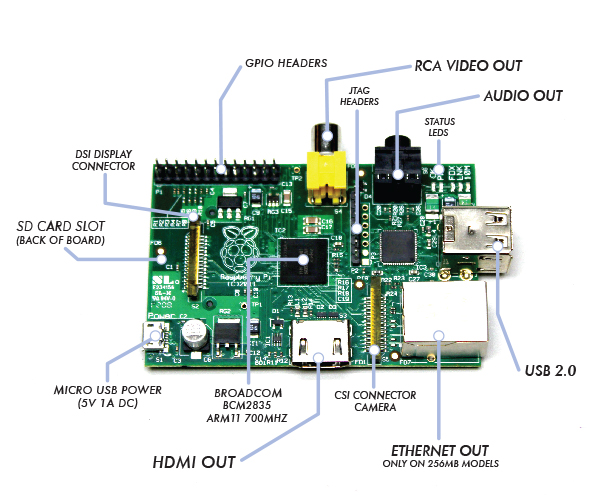
\includegraphics[width=0.7\textwidth]{graphics/Raspberry_Pi.png}	
    \caption{Raspberry Pi overview over peripherals}
    \label{fig:RPi}
\end{figure}

To control the Pi you can hook up a keyboard and a monitor directly to the board, or you can control it from another computer. 
This is achieved by using a SSH server on the Pi and a SSH client on the computer. 
SSH (Secure SHell) is a protocol that allows one computer to remotely control another via command line. A widely known program for doing this is PuTTY. To login over SSH, you need to know the IP-address of the host. This can be done by setting the IP-address static or to scan the network to find out which IP the Pi would have. Since both of these approaches are difficult on a big network like NTNU, we had to find another approach. The solution was to connect the Pi directly to the computer via an Ethernet cable. To do this we had to do some modifications, the full tutorial on how to do this see \footnote{\url{http://pihw.wordpress.com/guides/direct-network-connection/}}. To get internet access we first shared the Wi-Fi connection on the computer described here \footnote{\url{http://anwaarullah.wordpress.com/2013/08/12/sharing-wifi-internet-connection-with-raspberry-pi-through-lanethernet-headless-mode/}}. Later we used a Wi-Fi USB dongle. The driver for this dongle installed automatically and all we had to do was to configure \textit{/etc/network/interfaces}, and add the following:
\begin{verbatim}
    auto wlan0
    iface wlan0 inet dhcp
    wpa-ssid "<nameOfNetwork>"
    wpa-psk "<networkPassword>"
\end{verbatim}
We had to set up a own network to do this, because the eduroam network uses different setup.
\bigskip

\textbf{Raspberry Pi camera Module} \footnote{\url{http://www.raspberrypi.org/product/camera-module/}}
is a camera that can be used to take high-definition video. It communicates to the Pi over a ribbon cable connected to the CSI port (see image). We installed a Raspberry Pi Cam Web Interface by entering these commands
\begin{verbatim}
    git clone
    https://github.com/silvanmelchior/RPi_Cam_Web_Interface.git
    cd RPi_Cam_Web_Interface
    chmod u+x RPi_Cam_Web_Interface_Installer.sh
    ./RPi_Cam_Web_Interface_Installer.sh install
\end{verbatim}
from this website \footnote{\url{http://www.raspberrypi.org/forums/viewtopic.php?f=43&t=63276}}.
Remember to have the Pi updated and have installed git.
Video from the camera could we then watch in the browser by entering the IP-address of the Pi in the address field.
\bigskip

\textbf{Dynamixel AX-12 servomotors}
are motors that allows for precise control of angle and velocity. These motors are controlled over a half duplex UART, which is a byte oriented asynchronous serial communication protocol. You can control the motors and receive feedback by sending commands to it corresponding to the control table in the datasheet [PUT REFZ H3R3]. The most important features is the control of position and velocity. The servos can work like normal servos where you can put in the desired position, and a controller inside the servo will make the servo go to that position. This position is limited to between 0-300 degrees (see datasheet). The servo can also work in so called "Endless Turn" mode, where the servos can spin infinite. Here you can only control the velocity which the motors run. "Endless Turn" mode is activated by setting the angle limits (CW Angle Limit and CCW Angle Limit) to zero.
\bigskip

\textbf{Dynamixel AX-S1 Integrated Sensor}
is a sensor device capable of measuring sound, brightness, heat and distance to objects. It is also capable of making sound. The communication is the same as the servomotors and the sensor is connected to the same bus. 
\bigskip

\textbf{USB2Dynamixel} \footnote{\url{http://support.robotis.com/en/product/auxdevice/interface/usb2dxl_manual.htm}} is a USB device that allows the computer to create a virtual serial port (UART) and with some other circuitry, communicate with the servos over the USB port.
<<<<<<< HEAD
This USB requires no driver installation when running Linux, and since RaspBian is a Linux distro this simplifies things. 
=======
This USB requires no driver installation when running Linux, and since RaspBian is a Linux distribution this simplifies things. 
>>>>>>> eceb083a25ea2fab9e2a2ddc28da7565cf09b60b
The USB2Dynamixel is inserted into one of the USB ports on the Pi and the servo motors are connected to the device.

Since the Pi also has a hardware UART driver on two of its GPIO headers, we thought about if we could communicate with the servos through these pins. 
To do this we had to make the circuitry described on page 8 in the datasheet [PUT REFZ H3R3]. 
We would also have to implement our own code for the lower part of the communication (where we used a library from the manufacturer, more on that later).
UART is also widely supported by many lower end microcontrollers which don't have the support for an OS. 
Therefore using UART would mean that the code would be even more platform independent.
\bigskip

\textbf{Dynamixel SDK} is a programming library for controlling dynamixel servo motors. 
This library is available for Windows, Mac and Linux and easy to run on the Pi. 
Since the library is written in C it is easy to use it in this C++ project.
There is a great API reference \footnote{\url{http://support.robotis.com/en/software/dynamixelsdk.htm}} with the library.
The functions treat the lower part of the communication over USB2Dynamixel.
There are functions for initializing the communication, terminate the communication, sending byte and words (16 bit), receiving byte and words, and for ping. Ping is for checking if a device is connected.
There is also a page describing platform porting \footnote{\url{http://support.robotis.com/en/software/dynamixel_sdk/sourcestructure.htm}}


\subsection{The overall system of the robot}

\begin{figure}[H]
    \centering
    
\includegraphics[width=0.7\textwidth]{graphics/Robot_class_diagram.png}	
    \caption{Robot overall system}
    \label{fig:Class_diagram}
\end{figure}

This is how the overall system was made. It was our intention to make the system module based, such that it is easy to develop more things using the same modules. To make the modules we implemented classes in c++. That way you can make several motor, sensor, car or manipulator objects. 

The communication module was added because we used threads in our program. Since there are only one data-bus and therefore it can only be accessed by one thread, we had to implement \textit{Mutexes} such that only one thread can access the communication functions available in the dynamixel library at the time. \textit{Mutexes} are "locks" that protect such code blocks that can only be accessed by one at the time.

\subsection{Servo motors}

The first step is to make a servo motor move. 

\begin{figure}[H]
    \centering
    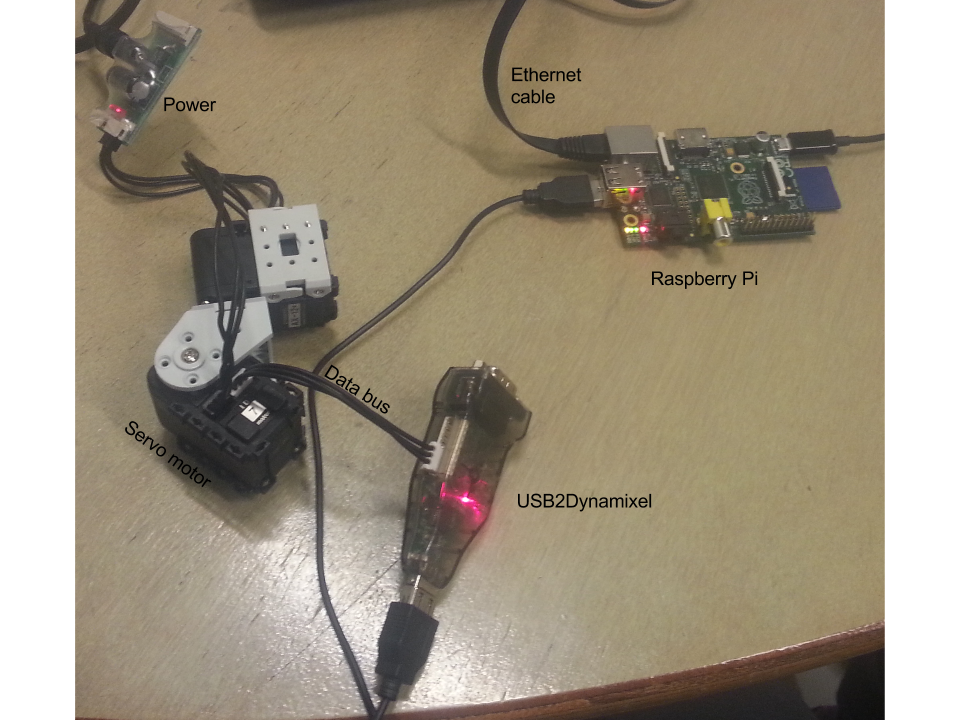
\includegraphics[width=0.7\textwidth]{graphics/Basic_oppsett.png}
    \caption{Servo motor test setup. The setup shows two motors, but that would not affect the code.}
    \label{fig:servo} 
\end{figure}

To make the servo motor move the example-program for the motor class could be used \footnote{LOCATION TO MOTOR EXAMPLE PROGRAM}. Alternative the example-file readWrite form the dynamixel library could be used \footnote{LOCATION TO READWRITE EXAMPLE FILE}. 
For this to work there are some important parameters which should be known:
\begin{itemize}
     \item ID - Each motor has its own ID. This way its possible to control which motor that should get the command. The ID need to be change in the code to the ID of the motor. If the motor ID is unknown, you could use the \textit{pingAll()} function. This will search for IDs on the bus, and print out those that are active
     \item Port - Which port the USB2Dynamixel is connected to. This is used to set up the communication to the motors. USB devices under Linux can be found under \textit{/dev/usb}. When testing we used deviceIndex = 0 (\textit{/dev/usb0}).
     \item Baudnumber - used to set the speed of the bus. This should always be one, which is 1Mbit/s, unless lower speeds are needed.
\end{itemize}
\bigskip

By replacing these parameters in the example file the servos should move back and forth when enter is pressed.


\subsection{Driving}
The next step is to make four wheels cooperate!
This was implemented in the class Car. Four servomotors are mounted under the base of the robot. The two motors on the right turns the same way and the two on the left turns the other way. When creating a car object all you have to do is write the IDs of the wheels. The motors are initialized in endless turn mode when the car object is created. There was functions for setting speed and turning the car both when the car is driving and when it had stopped. Turning the car was accomplished by setting the two right wheels one way, and the two left wheels the other way when the car had stopped. When the car was moving only one side was set to a lower speed to make the car turn while moving.


\begin{figure}[H]
    \centering
    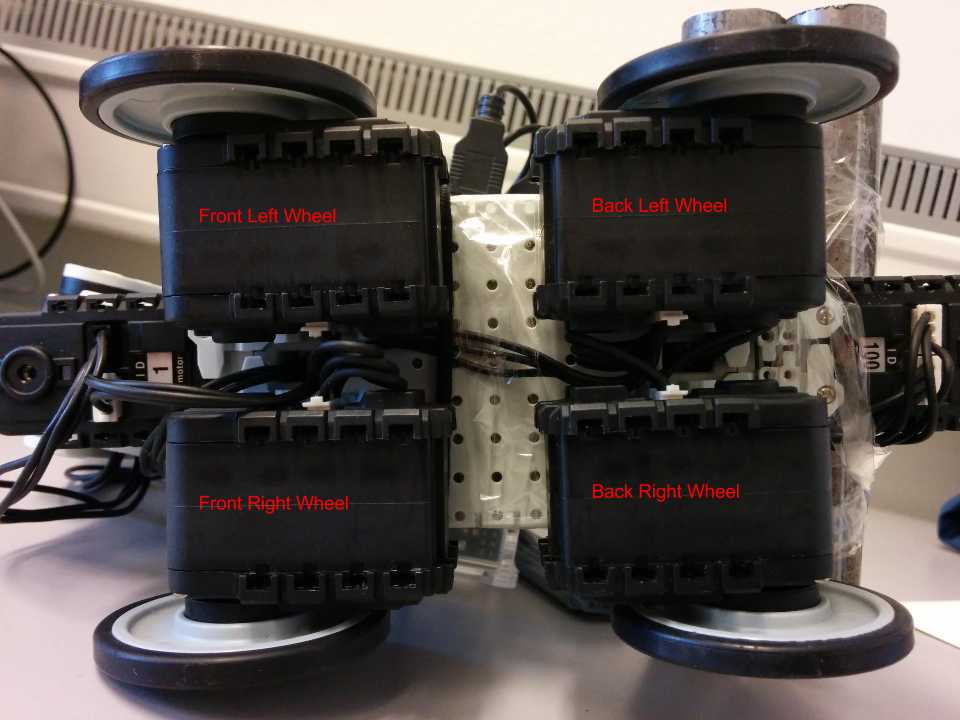
\includegraphics[width=0.7\textwidth]{graphics/Car.png}
    \caption{car overview}
    \label{fig:car} 
\end{figure}


In the example directory is an example program which demonstrates the car driving forward, backward and turning to left and right. The only thing needed are the IDs of the wheels. You can still use the pingAll() to check for IDs on the data-bus.

\subsection{Manipulator}

A manipulator was added to be able to pick up things and look around with the camera. The manipulator use three servomotors in the arm, and two in the gripper. The setup was like in the drawing below.

\begin{figure}[H]
    \centering
    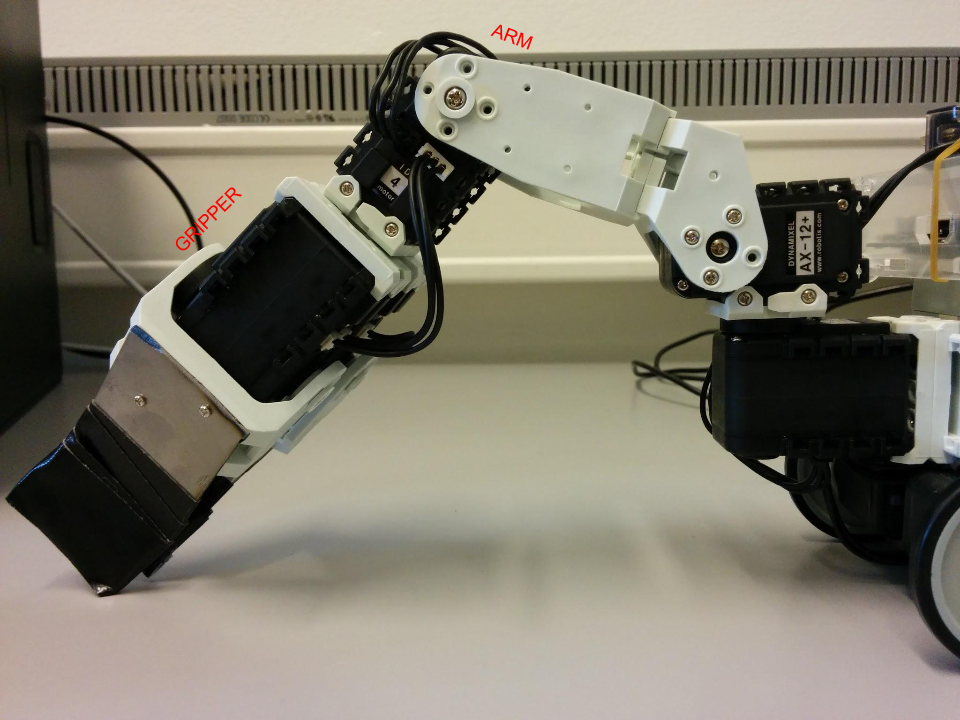
\includegraphics[width=0.7\textwidth]{graphics/Manipulator.png}
    \caption{manipulator overview}
    \label{fig:manipulator} 
\end{figure}

The class Manipulator implements the arm and the gripper.
\bigskip

\textbf{Arm}

The angles of the servomotors in the arm can be set directly by using the function setAngles($\theta_{1}$, $\theta_{2}$, $\theta_{3}$), or you can set the desired position in x, y and z, by using the function goToPosition(x,y,z). This function make use of inverse kinematic, with a geometric approach. 
The problem can be split up in to calculations, the calculation of $\theta_{2}$ and $\theta_{3}$, and the calculation of $\theta_{1}$. To calculate $\theta_{2}$ and $\theta_{3}$ we use the law of cosines.

\begin{figure}[H]
    \centering
    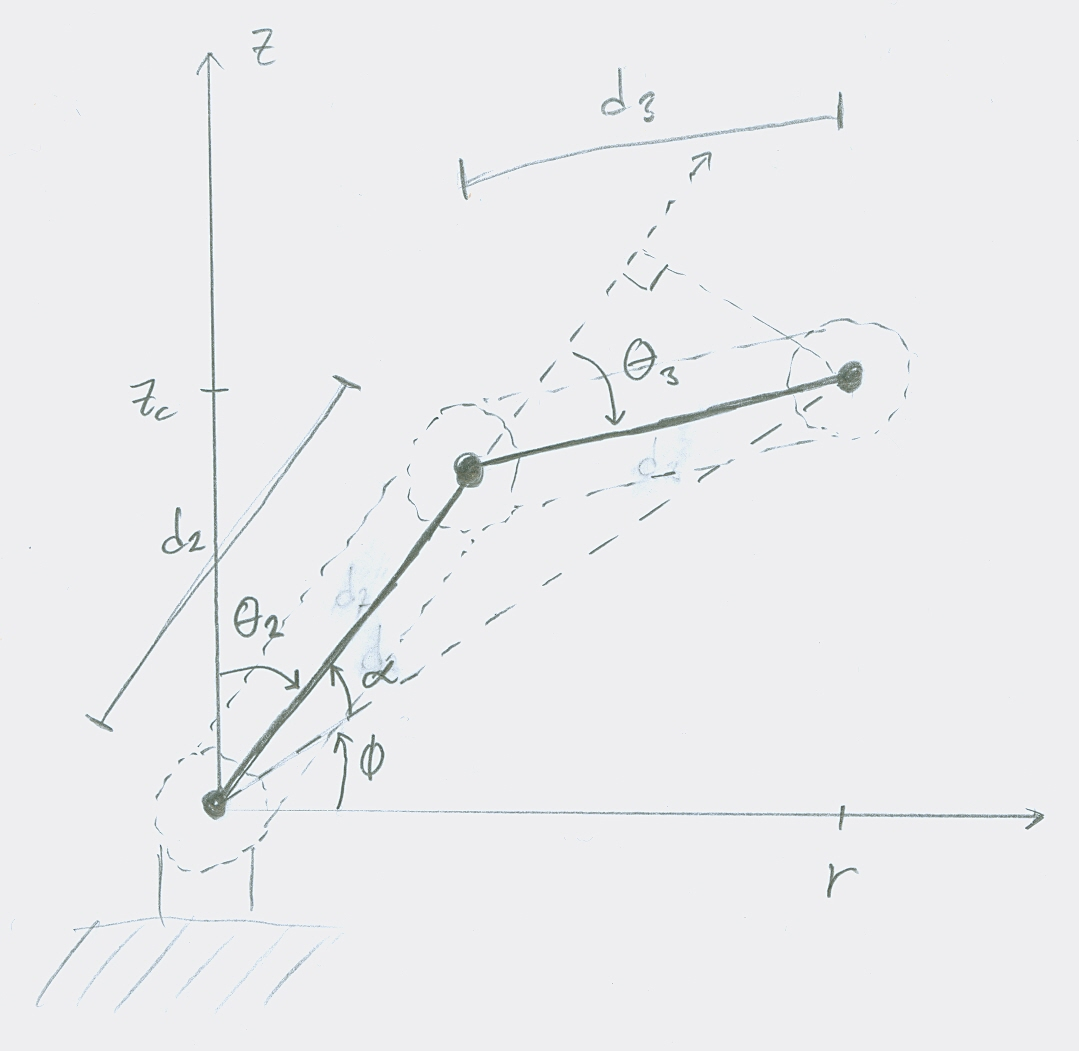
\includegraphics[width=0.7\textwidth]{graphics/Inverse_kinematic_1.jpg}	
    \caption{manipulator from the side}
    \label{fig:manipulator_side} 
\end{figure}

\begin{displaymath}
\begin{split}
-2d_{2}d_{3}\cos(\pi - \theta_{3}) = z_{c}^2 + r^2 - d_{2}^2 - d_{3}^2\\
r^2 = x_{c}^2 + y_{c}^2\\
\cos(\theta_{3}) = \frac{z_{c}^2 + x_{c}^2 + y_{c}^2 - d_{2}^2 - d_{3}^2}{2d_{2}d_{3}} = D\\
\sin(\theta_{3}) = \pm\sqrt{1-D^2}\\
\theta_{3} = \arctan(\frac{\pm\sqrt{1-D^2}}{D})
\\
\\
\theta_{2} = \frac{\pi}{2} - \alpha - \phi\\
\theta_{2} = \frac{\pi}{2} - \arctan(\frac{d_{3}\sin(\theta_{3})}{d_{2}+d_{3}\cos(\theta_{3})}) - \arctan(\frac{z_{c}}{r})
\end{split}
\end{displaymath}

Hence there are two solutions to the equation of $\theta_{3}$, one where $\theta_{3}$ is negative and one where $\theta_{3}$ is positive. The two solutions are called \textit{elbow up} and \textit{elbow down}. We chose the \textit{elbow up} solution because this would lead to less crashing with objects on the ground.
The length $d_{2}$ and $d_{3}$ had to be measured in mm and set in the code.

\begin{figure}[H]
    \centering
    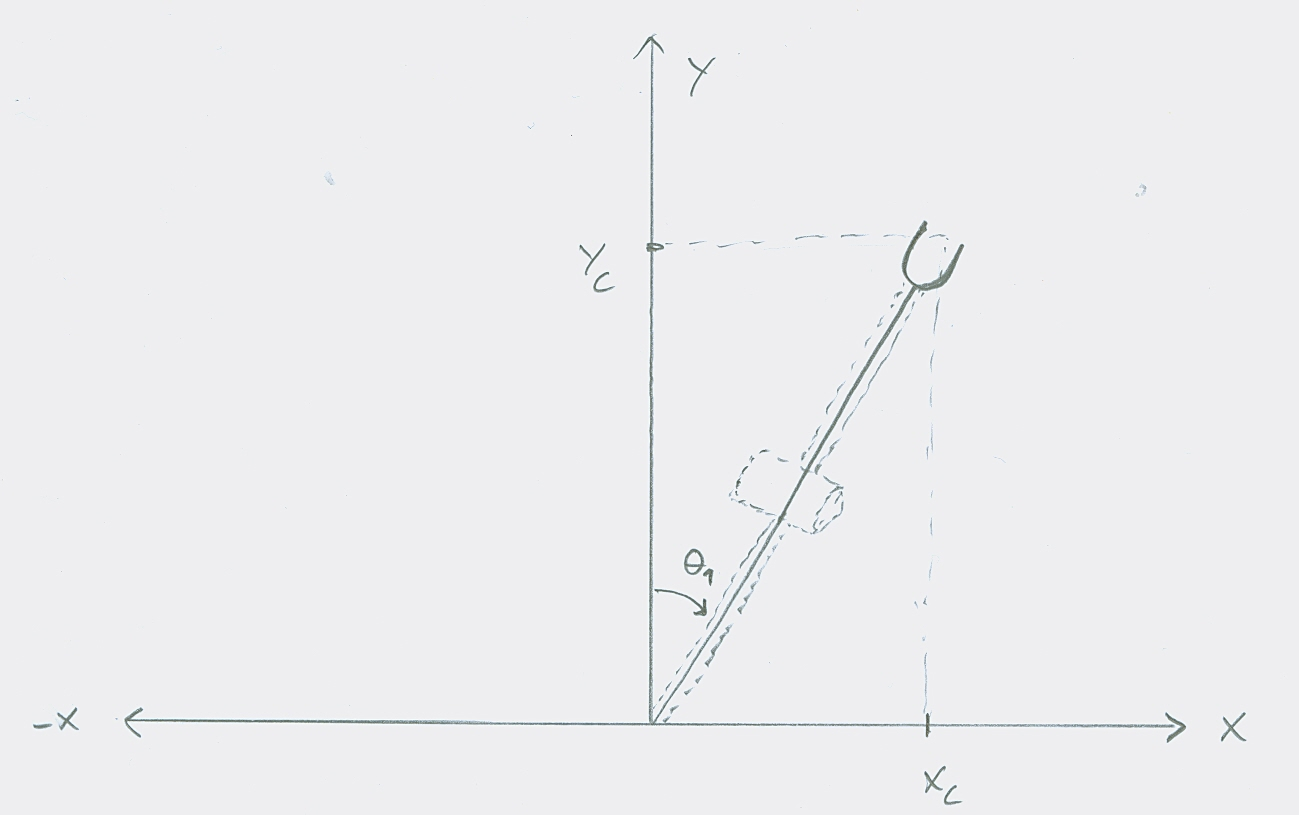
\includegraphics[width=0.7\textwidth]{graphics/Inverse_kinematic_2.jpg}
    \caption{manipulator from the top}
    \label{fig:manipulator_top} 
\end{figure}

The calculation of $\theta_{1}$ was simple.

$$\theta_{1} = \arctan(\frac{x_{c}}{y_{c}})$$

Since the servomotors only can move inside 0-300 degrees, the code had to include saturation limits on the angles, and will an error code if these limits are reached.
\bigskip

\textbf{Gripper}

The gripper used to servomotors on the end of the arm. The main problem with the gripper was to make it stop when it noticed it couldn't move further, and therefore not squeezing the object it had to grip. This was done by first setting the zero position where the two parts of the gripper could touch, and setting this as the first goal position. Then it had to read the position continuous until it noticed that it had reach the max number of consecutive reads. When this number was reached, the motors would stop ensuring that the object would not be destroyed.

\begin{figure}[H]
    \centering
    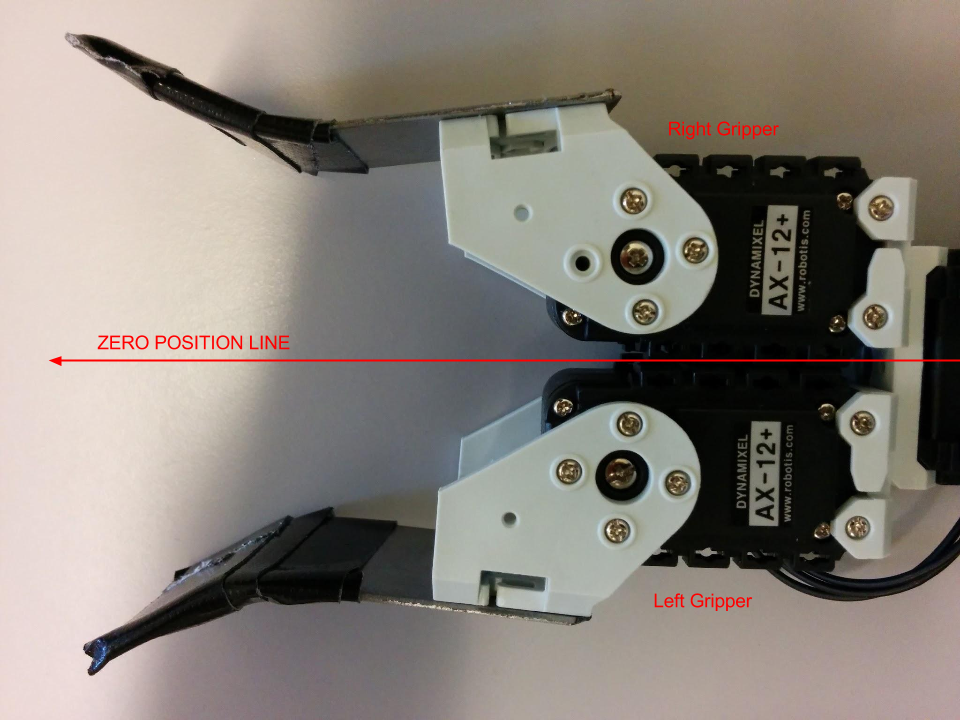
\includegraphics[width=0.7\textwidth]{graphics/Gripper.png}
    \caption{Gripper}
    \label{fig:gripper} 
\end{figure}

\bigskip

\textbf{Example}

The example file creates a manipulator with some given IDs and makes it move in y and z direction using inverse kinematic. It also demonstrates the gripper. The only thing needed are the IDs of the wheels. You can still use the pingAll() to check for IDs on the data-bus.

\subsection{Testing it all with a local interface}

One important feature of all system is to be able to test things at different levels. All of the modules are supplied with example-code testing the most basic functions. We thought that it would be nice to test all of the modules together without going through the internet. Then we wouldn't have problems of latency for example. 

The interface example program creates a window on the pi by using the X Window System. The window can detect mouse and keyboard input. To see the window you could hook up a monitor to the pi or you could use a program such as \textit{Xming}\footnote{\url{http://www.straightrunning.com/XmingNotes/}} which make it possible to open windows on the Raspberry Pi through the SSH connection. Explanation on how to do this is also explained here \footnote{\url{http://pihw.wordpress.com/guides/direct-network-connection/}} under step 3.

In the window that the program creates you could move the manipulator in the X-Y-plane by pushing the left mouse button and moving the mouse around. You can move up and down in z-direction by scrolling the wheel, and grab things with the gripper by pushing right mouse button. With w,s,a,d buttons you can drive  around.

The interface was very useful when debugging the hole program of the robot without the need of internet. Many problems arose due to the fact that there was much more communication on the bus, and due to other stress on the system. Also it was very pleasing to drive around and pick up things. 

\subsection{Sensor}

The use of the AX-S1 Integrated Sensor was realized by the Sensor class. Here are functions for calculating distance to objects using IR, functions for measuring light and functions for playing sound. Distance to objects are done by the sensor sending pulses with a IR-diode and measuring the strength of the IR returning. This way one can predict how close an object is (higher strength = close). 

The sensor can also play sound, either from its internal memory or by sending notes and how long it should play that note to it. In the datasheet is a table of notes and corresponding values. There are one function for each of these modes. The latter function takes in a array of notes and length of each note.

\subsection{Exception handling}

Another important feature of the setup of the robot is exception handling. We discovered that we often got error in communication when using the Dynamixel library. So we decided that there should be some kind of exception handling when the robot looses one of its motors or sensors. When one motor is lost it throws an exception with information on what went wrong and which motor it was. The exception can then be caught in the Car or Manipulator class and set the object in \textit{fail-safe} mode. When entering \textit{fail-safe} mode a thread is created that ping all the motors in the object regularly. This way the program will discover automatically when the object has recovered and set it in \textit{idle} mode again. One other way to do this would be to ping all the motors regularly and then also automatically discover when motors become unreachable. But this would make the data bus even more busy in \textit{idle} mode which may be undesirable and may cause more communication error.

When in \textit{fail-safe} mode the manipulator or car object disables all its functions. This way you can not for example drive the car if one wheel is lost, which would result in the car not driving straight forward. We thought about having a how we could operate the car when one wheel was gone. For example could we disable only the back wheels if just one of the back wheels was lost. We tried this and discovered that it was to much friction in the two wheels that the car wouldn't move at all, or not move in a straight line. Therefore we didn't choose this approach. 

For future work one could also think about how to implement a mode for operating the manipulator with one or more of the servomotors lost.

\subsection{Future problems/challenges}

As said in the last section future problems could be to implement a better \textit{fail-safe} mode where you could operate the car or manipulator even though one of the servomotors is lost.
\bigskip

Another problem with the code that we discovered is the use of threads together with the use of the Dynamixel library. To ensure that multiple threads wasn't speaking on the data bus at the same time, we had to introduce mutexes for the send and receive functions. The problem was with a the timeout in the Dynamixel library functions. If to long time pass before the functions receive something back on the bus, the functions would give an error back with the error command \textit{RXTIMEOUT}. The problem then arose if one thread sends something on the data bus waiting for a response, another thread takes over and when the thread that was sending come back again it has gone to long time, and it issues an error. This could be done by increasing the timeout in the Dynamixel function, which requires some knowledge on how the library works. 
A more elegant way is to make the communication functions \textit{atomic}, which would mean that no other thread could interrupt that thread when executing this line of code. %is this right?
\bigskip

The robot could be battery operated. Because the battery was quite dead we had to connect it to a power adapter. Also the Raspberry Pi was connected to the wall through an AC/DC adapter. With a better battery, one could make a circuit that also supplied the Pi through the battery, making the robot all cordless.
\bigskip

stream video to the internet instead of a local web server.

%more:
%main program thread sensor
%putting it all together main program in result?

%%% Local Variables: 
%%% mode: latex
%%% TeX-master: "../report"
%%% End: 

\section{Vehicle-server communication}
The vehicle needs a solid way of communicating with the server and other devices. We chose to use a server which hosts a rest API to acvhieve this. 
\begin{itemize}
    \item Raspberry Pi
    \item Dynamixel servomotors
    \item USB2Dynamixel
    \item Dynamixel SDK
\end{itemize}
\vspace{\secspace}

\textbf{Rasppberry Pi} (Pi) is a small single board computer. 
It has two USB inputs, ethernet, HDMI and gpio pins. 
This makes it the perfect prototyping computer for this kind of projects. 
The Pi is running its operating system from a SD card, and the OS is RaspBian which is a debian based linux distro. 
To controll the Pi a regular laptis is used. 
This is achieved by using a SSH server on the Pi and a SSH client on the computer. 
SSH (Secure SHell) is a protocol that allows one computer to remotely controll another via command line. 
\vspace{\secspace}

\textbf{Dynamixel servomotors}\footnote{\url{http://www.robotis.com/xe/dynamixel_en}} are motors that allows for precise controll of angle and velocity. 
These motors are controlled by three wires, power, gnd and signal. WRITE SOME MORE HERE!
\vspace{\secspace}

\textbf{USB2Dynamixel} is a USB device that allows easy controll of dynamixel servo motors. 
This USB requires no driver installation when running linux, and since RaspBian is a linux distro this simplifies things. 
The USB2Dynamixel is inserted into one of the USB ports on the Pi and the servor motors are connected to the device. 
\vspace{\secspace}

\textbf{Dynamixel SDK}\footnote{\url{http://support.robotis.com/en/software/dynamixelsdk.htm}} is a programming library for controlling dynamixel servo motors. 
This library is available for Windows, Mac and Linux and easy to run on the Pi. 
Since the library is written in C it is easy to use it in this C++ project. 

\subsection{Wiggle It}
The first step is to make a servo motor move. 
Since the USB device is linux compatible and the library also works in linux the Pi was used from the begining of the project. 
\begin{figure}[H]
    \centering
    %sett inn figure her
    \caption{fig:1servo}
    \label{Servo motor test setup} 
\end{figure}

To make the servo motor move an example c-file form the library was used\footnote{LOCATION TO EXAMPLE FILE}. 
For this to work there are som important parameters which should be known:
\begin{itemize}
     \item ID - Each motor has its own ID. This way its possible to control which motor that should get the command. 
     \item Port - Which port the USB2Dynamixel is connected to. This is used to set up the communication to the motors. 
     \item Mode - The servo motors can run in two different modes. Endless turn (like a wheel) and start2stop (from start position to specified position). 
\end{itemize}
\vspace{\secspace}

The servo motors used for this test had IDs 7 and 12, and can be found on the side of the servo. 
In linux the USB device can be found under /dev/usb, and using the Pi this device was /dev/usb0. 
By replacing this parameters in the example file two servos was wiggled. 


\subsection{Driving}
The next step is to make four wheels cooperate! 


\subsection{Future problems/challenges}
What happens if some of the wheels is disconnected? 
The answer for this question will not be covered in this report because of the timeframe, but it is an important issue that has to be resolved. 
The optimal solution is to find an algorithm that calculates the speed that the remaining wheels, so that the vehicle can obtain normal function even in failsafe mode. 
This will most likely depend on the surface under the vehicle. 


%%% Local Variables: 
%%% mode: latex
%%% TeX-master: "../report"
%%% End: 

\section{Security}
Concerns related to security were, as they typically are in this day and age, a thing.
Several issues arise as the platform allows users to control agents by issuing commands through a publicly available API, namely:

% Agent = active/connected robot/entity/thing
% user = bruker ja, ok?
% user client = bruker som tar i bruk webgrensesnittet
% server = serveren
% client = både agenter og user clients
\begin{enumerate}
	\item Restricting the execution of commands.
	\item Preventing replay of commands (replay attacks).
	\item Preventing others from masquerading as the server and spreading misinformation (man-in-the-middle type attacks).
\end{enumerate}
% jobbe deg oppover mot sluttresultatet

\subsection{Communication}
The server and clients communicate over the Hypertext Transfer Protocol layered on top of the SSL/TSL protocol. %TODO: insert reference to HTTPS/SSL/TLS
This is commonly known as ``HTTPS''.
The API server enforces the use of HTTPS and refuses to serve requests over regular HTTP.
This means that all communication between the server and clients is encrypted, which prevents attackers from eavesdropping on the communication.



While these guarantees of security 
All these ``security guarantees'' depend on the various  
Barring weaknesses or exploits in HTTPS or any of the underlying protocols or infrastructure

%TODO: find reference for SSL/TLS Certificate thing type deal
%TODO: find a paper or whatever (RFC?) on HTTPS and SSL/TLS

\subsection{Identity}
In HTTPS, X.509 certificates are employed to guarantee the identity of the server.
%TODO: Insert reference to x.509 certificates
This prevents attackers from trivially impersonating the server.
An attacker might want to impersonate the server in order to serve users faulty sensor data or collect a large amount of cipher texts in order to exploit a potential weakness in the signature scheme in the hopes of obtaining a user's private key.

\subsection{Access restriction}
Access Control Lists, in addition to a user registration system, could be used to restrict access to certain commands.
There would be an access control list for each agent registered in the system, and its owner(s) would be able to edit it in order to grant or deny other users access to the agents' functions.
Users could either be explicitly granted access rights or denied them.

This would, coupled with a method of identifying the user from which a request originated from, prevent un-authorized execution of commands to the agents.
At least in theory, given that the access control lists are properly maintained by the agents' owners.
An example of ``improper maintenance'' could be that the owners, wishing that no one besides themselves be allowed to issue commands to their agents, explicitly deny access to each and every other registered user while neglecting to deny access to non-users (i.e. non-registered users, the general public).

%TODO: reference ACL
%https://www.cs.cornell.edu/courses/cs513/2007fa/NL.accessControl.html

\subsection{User identification}
To identify users one could require them to register themselves with an unique username or ID on a website, and further require that they submit a public key.
Users wanting to access restricted commands or API-calls would then sign their requests using their private key and submit their unique username or ID along with the request.
The username or ID would be used to identify the user's public key, which would be used to verify the signature attached to the request.

% refere til github sin implementasjon av dette?

% kanskje et avsnitt om PKI?
% Herp derp users can be required to leave a public key on our servers and to sign any commands or API-calls that are access restricted with their private key
% we can then use their public key to verify that the request was sent by given user 

\subsection{Other security related issues}
While our system can claim certain to possess certain security guarantees, these are in effect by the virtue of the underlying implementations.
Even if the underlying mathematics of whatever encryption or security protocol has been proven to be secure, faults or exploits could be found in the implementations.

For example, on the 7th of April 2014, a vulnerability in several newer versions of OpenSSL was made public.
%TODO: reference http://www.openssl.org/news/secadv_20140407.txt
This vulnerability, nicknamed ``Heartbleed'', allowed remote attackers to obtain sensitive information (e.g. the server's private key) from web servers running the affected versions of OpenSSL.
%TODO: Reference to http://heartbleed.com/
This is an example of an implementation vulnerability.
Even if the theory is sound, the implementation might not be.
There is little possibility of safeguarding entirely against such eventualities -- even if one uses the more stable and secure versions of a program or software, there might exist vulnerabilities unknown to the public.
%TODO: reference to OpenSSL



% Result
\chapter{Results}
We should have like, a graph or drawing of the finished system here shouldn't with the involved components and actors and what gets transferred between them.
Like those drawings Anders have been keeping safe in his lockerbox or whatever.


The project was initially split into three parts. These were ``server'',``agent(robot)'' and ``server-agent communication''. 
At the concluding phase of the project, these three part were combined to form the whole system.
The planning work done early proved to be very good, as the finishing phase went surprisingly smooth. 
The server part was augmented with a graphical user interface, which can be used from any web browser. 
It can be accessed by both smartphones and computer, and from anywhere in the world. 
The robot's wheels and arm was successfully controlled via this interface. 
The latency was tolerable for controlling the vehicle, but the system can in no way guarantee real time performance.
The worst case agent-server latency is too high for this.
The robot's error handling worked well, as its behavior was as intended when we introduced various error conditions.



% Conclusion
\chapter{Conclusion}
There should be some, like, text here.
Probably.
Summarizing what we got done and what kind of future work exists.
Like "recommended avenues for future research."
Oooh we should mention that the system can be used as the basis for a web service (like github) or on a local network to allow the remote control of devices on it (but not from the outside, like idk maybe a company would want to do this).
The great thing is that once you've written the agent-client and user-client you can re-use these on other platforms.


% References
\bibliography{}{}


\end{document}
